\documentclass{standalone}
\usepackage{pgfplots}
\pgfplotsset{compat=newest}

\begin{document}
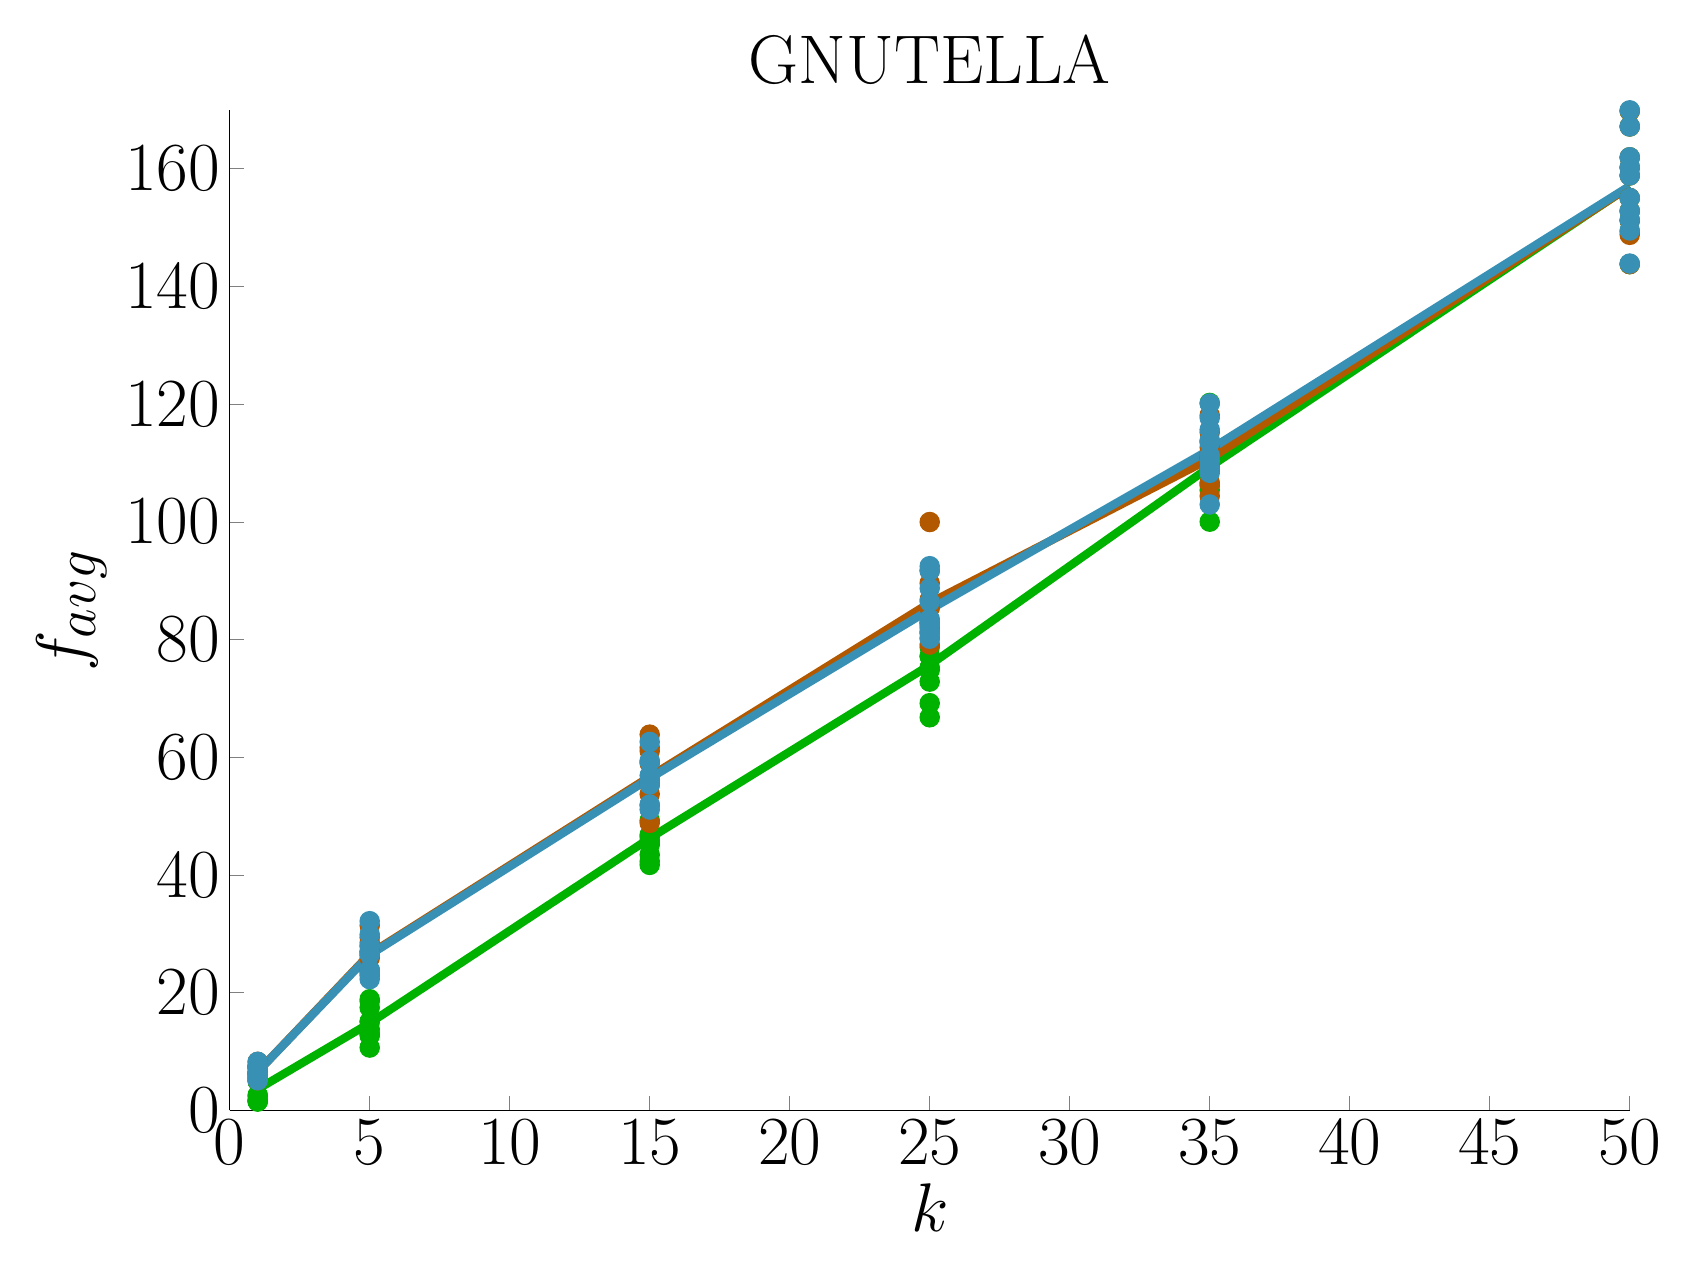
\begin{tikzpicture}

\begin{axis}[%
title style={font=\Huge},
title=GNUTELLA,
tick label style={font=\Huge},
label style={font=\Huge},
legend style={font=\Huge},
view={0}{90},
max space between ticks=50pt,
width=7in,
height=5in,
scale only axis,
xmin=0, xmax=50,
%xtick={0, 20, 40, 60, 80, 100},
xlabel={$k$},
ymin=0, ymax=169.92,
ylabel={$f_{avg}$},
major tick length=5pt,
axis lines*=left,
legend cell align=left,
clip=false]

\addplot [
only marks,
mark=*,
mark size=3.5pt,
color=green!70!black,
%solid,
%line width=2pt,
]
coordinates{
(1,1.48)(1,1.54)(1,1.72)(1,1.74)(1,2.4)(1,2.6)(1,4.9)(1,5.6)(1,6.4)(1,7.5)(5,10.66)(5,12.68)(5,12.98)(5,13.04)(5,13.78)(5,15.04)(5,15.1)(5,17.44)(5,18.54)(5,18.88)(15,41.7)(15,42.32)(15,43.42)(15,45.12)(15,45.44)(15,45.86)(15,46.46)(15,46.8)(15,49.26)(15,55.96)(25,66.78)(25,69.18)(25,72.84)(25,74.8)(25,75.24)(25,77.14)(25,77.18)(25,78.7)(25,81.96)(25,82.68)(35,100.02)(35,105.38)(35,106.12)(35,108.76)(35,109.1)(35,109.2)(35,110.08)(35,110.72)(35,113.68)(35,120.2)(50,143.78)(50,149.3)(50,151.2)(50,152.82)(50,155.02)(50,158.86)(50,160.22)(50,161.92)(50,167.18)(50,169.8)
};

\addplot [
only marks,
mark=*,
mark size=3.5pt,
color=orange!70!black,
%solid,
%line width=2pt,
]
coordinates{
(1,5.1)(1,5.36)(1,5.84)(1,6.2)(1,6.26)(1,6.52)(1,7.12)(1,7.4)(1,7.5)(1,8.24)(5,22.88)(5,23.68)(5,23.7)(5,25.88)(5,26.34)(5,26.94)(5,27.0)(5,28.48)(5,29.38)(5,31.4)(15,48.84)(15,51.8)(15,53.72)(15,55.34)(15,55.82)(15,55.88)(15,58.98)(15,61.06)(15,61.66)(15,63.84)(25,79.14)(25,80.26)(25,81.08)(25,82.88)(25,85.4)(25,85.44)(25,86.76)(25,89.58)(25,91.7)(25,99.96)(35,104.38)(35,106.42)(35,106.66)(35,109.88)(35,110.78)(35,111.1)(35,111.72)(35,112.66)(35,115.22)(35,118.1)(50,143.78)(50,148.76)(50,151.2)(50,152.82)(50,155.02)(50,158.86)(50,160.22)(50,161.92)(50,167.18)(50,169.8)
};

\addplot [
only marks,
mark=*,
mark size=3.5pt,
color=cyan!70!black,
%solid,
%line width=2pt,
]
coordinates{
(1,5.1)(1,5.36)(1,5.84)(1,6.2)(1,6.26)(1,6.52)(1,7.12)(1,7.4)(1,7.5)(1,8.24)(5,22.28)(5,23.24)(5,23.66)(5,23.88)(5,26.48)(5,26.74)(5,27.86)(5,27.98)(5,29.9)(5,32.14)(15,51.1)(15,51.96)(15,55.36)(15,55.48)(15,56.08)(15,56.08)(15,56.88)(15,59.2)(15,59.38)(15,62.6)(25,80.14)(25,81.16)(25,81.4)(25,82.32)(25,82.88)(25,83.48)(25,86.42)(25,88.72)(25,91.68)(25,92.46)(35,102.94)(35,108.32)(35,109.1)(35,110.32)(35,111.26)(35,113.44)(35,113.82)(35,115.66)(35,117.66)(35,120.1)(50,143.88)(50,149.5)(50,151.28)(50,152.82)(50,155.02)(50,158.86)(50,160.26)(50,161.94)(50,167.18)(50,169.92)
};
p
\addplot [
color=green!70!black,
solid,
line width=3pt
]
coordinates{
(1,3.588)(5,14.814)(15,46.234)(25,75.65)(35,109.326)(50,157.01)
};

\addplot [
color=orange!70!black,
solid,
line width=3pt
]
coordinates{
(1,6.554)(5,26.568)(15,56.694)(25,86.22)(35,110.692)(50,156.956)
};

\addplot [
color=cyan!70!black,
solid,
line width=3pt
]
coordinates{
(1,6.554)(5,26.416)(15,56.412)(25,85.066)(35,112.262)(50,157.066)
};


\end{axis}
\end{tikzpicture}
\end{document}
